\section{Datasets}\label{sec:datasets}

% Stories: 97828 docs, 4476098 words
% Abstracts: 181759 docs, 27884893 words
% Lyrics: 1741697 docs, 57623316 words
\begin{itemize}[leftmargin=*,label=-]
    \item \stories{} ($100$K examples, $5$M words) \\
    Short stories from the ROCStories dataset \citep{mostafazadeh2016corpus}. Each story contains a title and five sentences.
    \item \abstracts{} ($200$K examples, $30$M words) \\
    Abstracts from CS papers on arXiv
    \item \lyrics{} ($2$M examples, $60$M words) \\
    Song lyrics from \url{lyrics.com}
\end{itemize}

\noindent We experimented on multiple datasets to demonstrate that our framework was not custom tailored to a single domain. 
On the \stories{} and \abstracts{} datasets, we include metadata (story title, paper subject matter, etc.), as the first ``paragraph'' of the document. 
By providing these paragraphs (\Cref{sec:mask_deets}), our infilling model implicitly learns to summarize (e.g. infill a title given a story), and do conditional generation (e.g. infill a story given a title).
On the \lyrics{} dataset, infilling models may be especially helpful to humans; external aid in the form of rhyming dictionaries is already commonly employed in this domain.

To ensure that all experiments were trained on the same data,
we removed infilling examples which would have exceeded our training sequence length of $256$ tokens for the model with the longest sequence length (\lmall{}). 
This removed no examples from \stories{}, a small fraction of examples from \lyrics{}, and a substantial number of examples from \abstracts{}. 

\section{Masking function}\label{sec:mask_deets}

We design a mask function which takes the entire document and selectively masks several span granularities: words, $n$-grams, sentences, paragraphs, and entire documents. 
Accordingly, models trained via ILM on this masking function offer users the ability to specify the granularity of text to infill at a particular location. 
This allows users to have coarse but intuitive control over infilling length, so that multiple paragraphs are not generated when the user was expecting a single word.

Our masking function first constructs a tree of the training example (using the natural hierarchy of documents, paragraphs, sentences, and words). 
Then, using a pre-order tree traversal, each subtree is masked with $3\%$ probability (or ignored if any of its ancestors are already masked).
If the entire document (root node of the tree) is masked, then the infilling model's job is equivalent to that of a language model. 
If a word (leaf) is selected to be masked, $50\%$ of the time we mask that individual word, otherwise we mask an $n$-gram of random length between $1$ and $\min(8, \text{\# words left in the sentence})$ words (inclusive). 
Note that a word may comprise multiple tokens, as GPT-2 uses sub-word tokenization~\citep{sennrich2015neural}.
We chose the value of $3\%$ as, for the datasets we considered, it resulted in a marginal token mask rate of around $15\%$, echoing the configuration of~\citet{devlin2019bert}.

We add special tokens for each granularity to our model's vocabulary (e.g. \blankword), 
so that the user may specify which granularity they would like the infilling model to produce.
This functionality can be explored in our demo: \url{https://chrisdonahue.com/ilm}.

While we focus on this specific mask function in this paper, 
we structured the ILM codebase to allow users to train infilling models for completely different use cases. 
Users need only define a new mask function which takes complete documents and outputs lists of character-level spans representing the desired spans to be masked.

\section{Hyperparameters}\label{sec:hyperparams}

We use early stopping based on the PPL of the model on infilling the masked token for the validation set. 
We train all models using the default fine-tuning parameters specified in the \texttt{transformers} library~\citep{wolf2019transformers}, except that we use a batch size of $24$ and a sequence length of $256$. 

Note that the most straightforward way of training an LM on ILM examples (\Cref{sec:training}) is to maximize the likelihood of the entire concatenated example: $\xtilde$, $\text{\sep}$, and $\y$. 
This trains the model to predict tokens in $\xtilde$ even though such behavior is not necessary at inference time as $\xtilde$ will always be fully-specified. 
Nevertheless, we found that this additional supervision \emph{improved} performance when evaluating model PPL of $\y$. 
Conveniently, this is also the default behavior when adapting existing LM training code for use with ILM.

\section{Evaluation on language modeling and infilling other granularities}\label{sec:eval_granularities}

Our quantitative evaluation (\Cref{sec:statistical}) examined the sentence infilling performance of GPT-2 initialized from the large-scale pre-trained checkpoint after fine-tuning on different datasets and infilling strategies. 
Here, we report PPL for GPT-2 both initialized from scratch and from the pre-trained checkpoint for several other configurations: language modeling, a mixture of granularities, specific granularities, and language modeling.

\subsection{Language modeling}\label{sec:quant_lm}

\begin{table}[t]
    \centering
    \begin{tabular}[t]{lccc}
        \toprule
            & \sto{}   & \abs{}   & \lyr{} \\
        \midrule
\lmscratch{} & 33.4 & 52.1 & 25.1 \\
\lmrevscratch{} & 32.9 & 53.9 & 24.7 \\
\lmallscratch{} & 30.4 & 44.6 & 26.2 \\
\ilmscratch{} & 30.8 & 45.3 & 30.6 \\
\lm{} & 17.6 & 25.7 & 20.8 \\
\lmrev{} & 25.1 & 36.7 & 23.7 \\
\lmall{} & 17.8 & 25.2 & 21.5 \\
\ilm{} & 18.1 & 23.9 & 23.0 \\
        \bottomrule
    \end{tabular}
    \caption{Document infilling PPL (or language modeling) of ILM and baselines initialized either from scratch or from the pre-trained checkpoint across three datasets. Note that PPL of \ilm{} is similar to \lm{}, implying that our infilling strategy can reasonably maintain the ability to perform language modeling while extending the ability to infill.}
    \label{tab:granu_ppl_documents}
\end{table}

In~\Cref{tab:granu_ppl_documents}, we report PPL for ``document infilling,'' which is equivalent to language modeling (because $\xtilde$ is always \blankdocument{}). 
Because of how we structured our mask function (\Cref{sec:mask_deets}), 
$3$\% of infilling examples consist of the entire document masked out, 
which results in the ability of our ILM framework to perform standard infilling. 
We see that performance of \ilm{} is similar to that of \lm{} on this task, even though \ilm{} sees far fewer examples of language modeling compared to \lm{}.

\subsection{Mixture of granularities}

\begin{table}[t]
    \centering
    \begin{tabular}[t]{lccc}
        \toprule
            & \sto{}   & \abs{}   & \lyr{} \\
        \midrule
\lmscratch{} & 34.0 & 52.8 & 28.9 \\
\lmrevscratch{} & 34.9 & 59.3 & 30.4 \\
\lmallscratch{} & 27.0 & 46.2 & 24.3 \\
\ilmscratch{} & 25.5 & 46.0 & 27.5 \\
\lm{} & 17.5 & 25.5 & 23.9 \\
\lmrev{} & 26.5 & 39.0 & 29.2 \\
\lmall{} & 15.1 & 24.4 & 19.3 \\
\ilm{} & 14.9 & 23.5 & 20.2 \\
        \bottomrule
    \end{tabular}
    \caption{Mixture infilling PPL of all models (a mixture of all granularities).}
    \label{tab:granu_ppl_all}
\end{table}

In \Cref{tab:granu_ppl_all}, we report results for a mixture of granularities. 
Specifically, we run the same mask function we use for training (\Cref{sec:mask_deets}) on our test data and evaluate PPL on the masked spans.
This reflects general infilling ability across a wide variety of granularities (and hence lengths). 
Unlike our other quantitative evaluations, there may be multiple variable-length spans missing from each example in this evaluation.
Results are similar to that of sentence infilling. 
Namely, that \ilm{} outperforms \lm{} and \lmrev{} and is similar to \lmall{} despite using much less memory.

\subsection{Individual granularities}

\begin{table}[t]
    \centering
    \begin{tabular}[t]{lccc}
        \toprule
            & \sto{}   & \abs{}   & \lyr{} \\
        \midrule
\lmscratch{} & 35.6 & 51.5 & 25.1 \\
\lmrevscratch{} & 34.8 & 65.1 & 24.7 \\
\lmallscratch{} & 33.4 & 45.0 & 26.2 \\
\ilmscratch{} & 34.3 & 45.3 & 30.6 \\
\lm{} & 18.3 & 24.2 & 20.8 \\
\lmrev{} & 26.5 & 42.8 & 23.7 \\
\lmall{} & 20.4 & 23.4 & 21.5 \\
\ilm{} & 20.7 & 22.5 & 23.0 \\
        \bottomrule
    \end{tabular}
    \caption{
    % On paragraph infilling, PPL of all models across all datasets.
    Paragraph infilling PPL of all models.
    }
    \label{tab:granu_ppl_paragraphs}
\end{table}

\begin{table}[t]
    \centering
    \begin{tabular}[t]{lccc}
        \toprule
            & \sto{}   & \abs{}   & \lyr{} \\
        \midrule
\lmscratch{} & 36.0 & 65.4 & 33.5 \\
\lmrevscratch{} & 35.1 & 92.2 & 35.8 \\
\lmallscratch{} & 27.1 & 53.8 & 27.1 \\
\ilmscratch{} & 26.7 & 51.0 & 31.0 \\
\lm{} & 18.3 & 27.9 & 27.7 \\
\lmrev{} & 27.1 & 46.5 & 34.3 \\
\lmall{} & 15.6 & 22.3 & 21.4 \\
\ilm{} & 15.6 & 22.4 & 22.6 \\
        \bottomrule
    \end{tabular}
    \caption{Sentence infilling PPL of all models.}
    \label{tab:granu_ppl_sentences}
\end{table}

\begin{table}[t]
    \centering
    \begin{tabular}[t]{lccc}
        \toprule
            & \sto{}   & \abs{}   & \lyr{} \\
        \midrule
\lmscratch{} & 36.1 & 62.5 & 34.1 \\
\lmrevscratch{} & 36.4 & 89.1 & 36.3 \\
\lmallscratch{} & 26.4 & 60.1 & 24.3 \\
\ilmscratch{} & 23.1 & 49.5 & 26.3 \\
\lm{} & 19.2 & 25.5 & 28.2 \\
\lmrev{} & 26.6 & 45.0 & 34.8 \\
\lmall{} & 14.5 & 20.5 & 18.6 \\
\ilm{} & 13.8 & 21.5 & 18.8 \\
        \bottomrule
    \end{tabular}
    \caption{N-gram infilling PPL of all models.}
    \label{tab:granu_ppl_ngrams}
\end{table}

\begin{table}[t]
    \centering
    \begin{tabular}[t]{lccc}
        \toprule
            & \sto{}   & \abs{}   & \lyr{} \\
        \midrule
\lmscratch{} & 32.3 & 57.2 & 34.8 \\
\lmrevscratch{} & 31.6 & 100.0 & 36.7 \\
\lmallscratch{} & 12.6 & 51.8 & 12.5 \\
\ilmscratch{} & 9.2 & 37.9 & 12.2 \\
\lm{} & 17.1 & 23.0 & 28.7 \\
\lmrev{} & 24.1 & 45.0 & 35.1 \\
\lmall{} & 7.5 & 15.8 & 9.5 \\
\ilm{} & 5.4 & 14.2 & 8.5 \\
        \bottomrule
    \end{tabular}
    \caption{Word infilling PPL of all models.}
    \label{tab:granu_ppl_words}
\end{table}


In \Cref{tab:granu_ppl_paragraphs,tab:granu_ppl_sentences,tab:granu_ppl_ngrams,tab:granu_ppl_words} we report PPL values for infilling performance on paragraphs, sentences, n-grams, and words, respectively, across the three datasets. 

For each granularity, we create one infilling example per document from the test set with exactly one masked span (randomly chosen from all spans of that granularity for that document).
Then, we compute PPL only on the tokens which comprise the masked span, i.e., PPL is computed for all models on exactly the same set of tokens.
Across all granularities, we observe that \ilm{} outperforms \lm{} and \lmrev{} and either outperforms or is comparable with \lmall{} while using less memory.

\section{Details on human evaluation}\label{sec:human_eval_details}\label{sec:more_examples}

For human evaluation, we sampled 100 stories from the test set of the \stories{} dataset. 
From each story, we masked out one sentence at a time, thereby resulting in 500 stories with masked sentences. 
Then we used these stories as context and tasked each model with infilling the masked sentence. 

We compared 8 models in total. 
In addition to the four models reported in \Cref{sec:human} (BERT, SA, LM, and ILM), we included the models which are initialized from scratch (as opposed to initialized from the large-scale pre-trained checkpoint) for exhaustive comparison.
Furthermore, to filter out spam, we used a control model which always generates ``This sentence was generated by a computer.''
Lastly, we included the original sentence from the dataset as a reference model (Human) to sanity check the max score is around 80\%.

Each annotator was shown 8 stories, one from each model, and was asked to identify one of the five sentences generated by machine (see \Cref{fig:amt_example} for an example). 
Among the 100 collected responses, we filtered out 5 responses whose annotation for the control model was wrong. 
The quantitative and qualitative results can be found in \Cref{tab:human_eval_all} and \Cref{fig:more_examples}, respectively.
All model outputs and responses of human evaluation can be found at \url{https://github.com/chrisdonahue/ilm}.
% CHRIS: I changed this to point to the github instead of Google Drive so that we can change the link if we need to in the future.


\begin{table}[ht]
    \centering
    \begin{tabular}[h]{lc}
        \toprule
         & Score (\%) \\
        \midrule
        Control & 0 \\
        BERT & 20 \\
        SA & 29 \\
        LM (scratch) & 40 \\
        LM & 41 \\
        ILM (scratch) & 39 \\
        ILM & 45 \\
        Human & 78 \\
        \bottomrule
    \end{tabular}
    \caption{Human evaluation results.}\label{tab:human_eval_all}
\end{table}

\begin{figure}[ht]
    \centering
    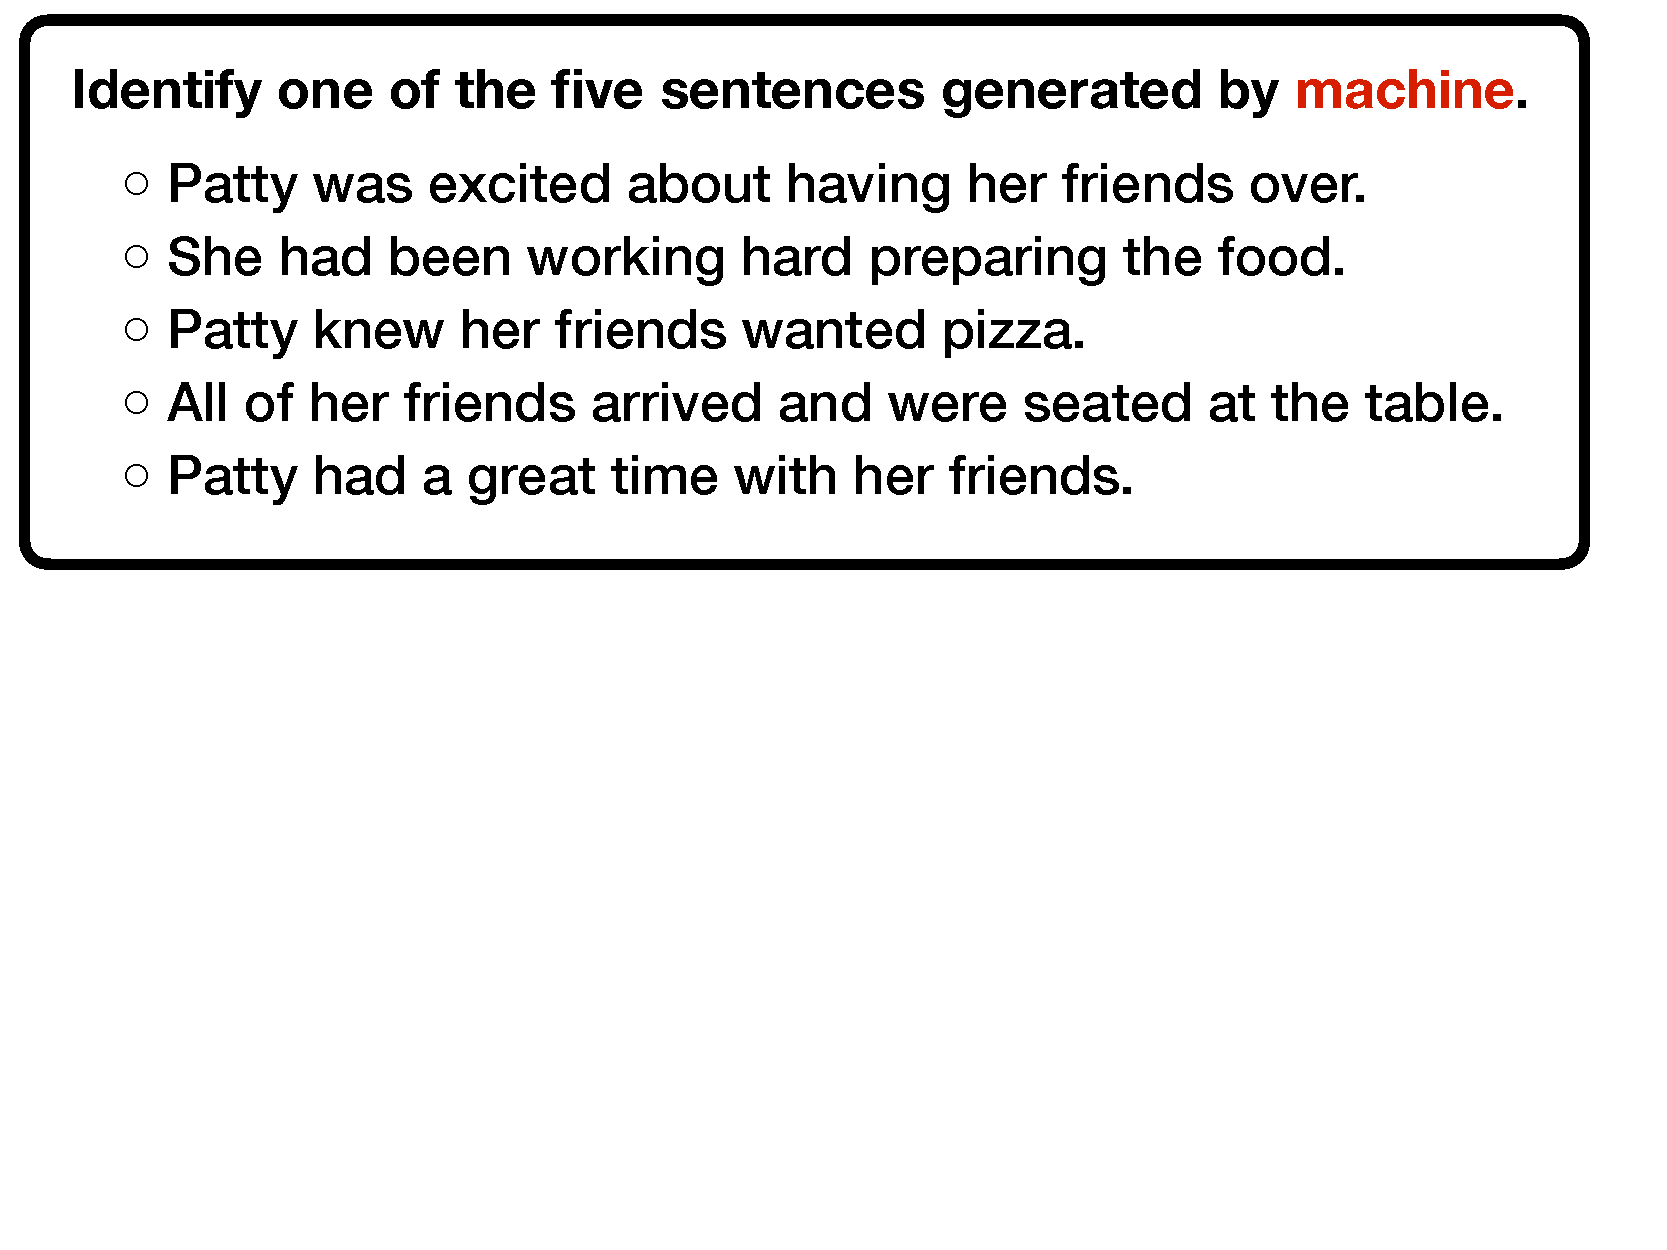
\includegraphics[width=1\linewidth]{figures/ilm_interface.pdf}
    \vspace{-3.5cm}
    \caption{Example of a task and instruction for human evaluation on Amazon Mechanical Turk.}\label{fig:amt_example}
\end{figure}

\begin{figure}[h]
\centering
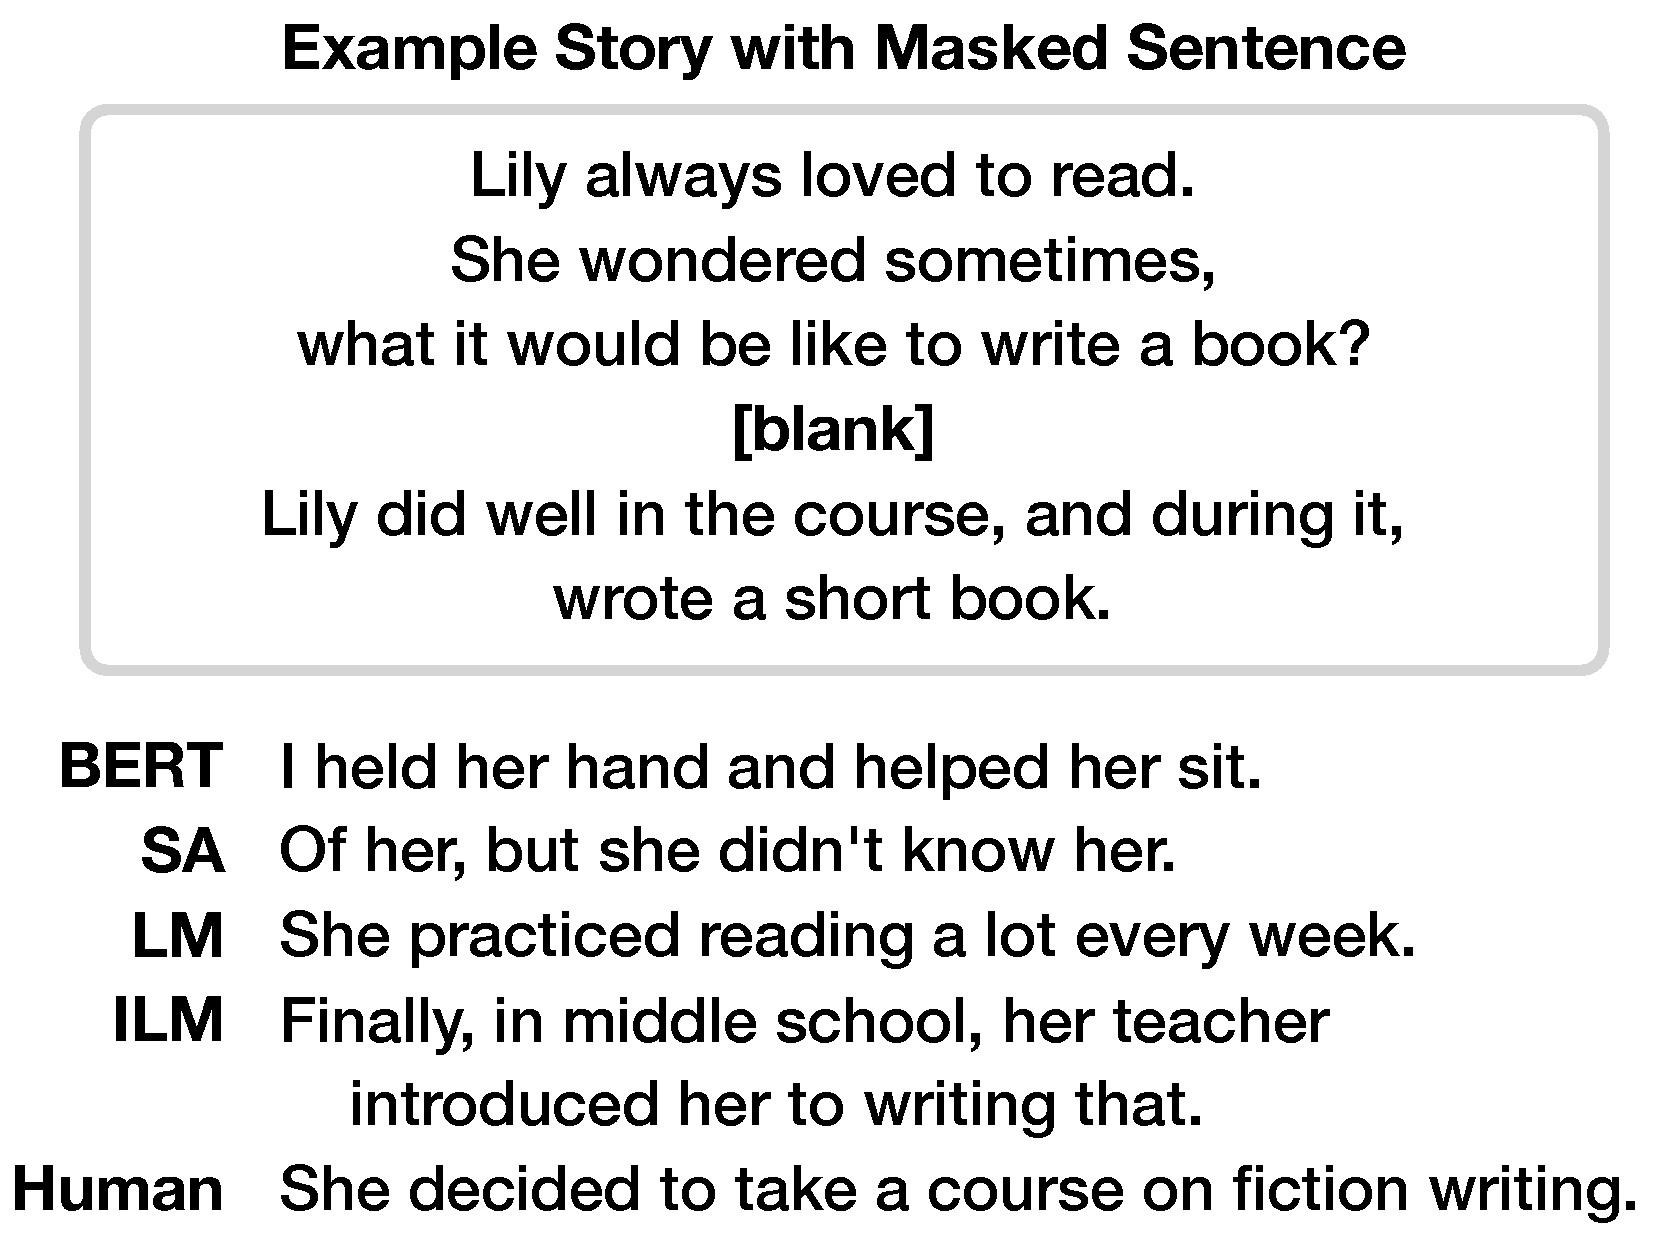
\includegraphics[width=1\linewidth]{figures/ilm_example_story1.pdf}
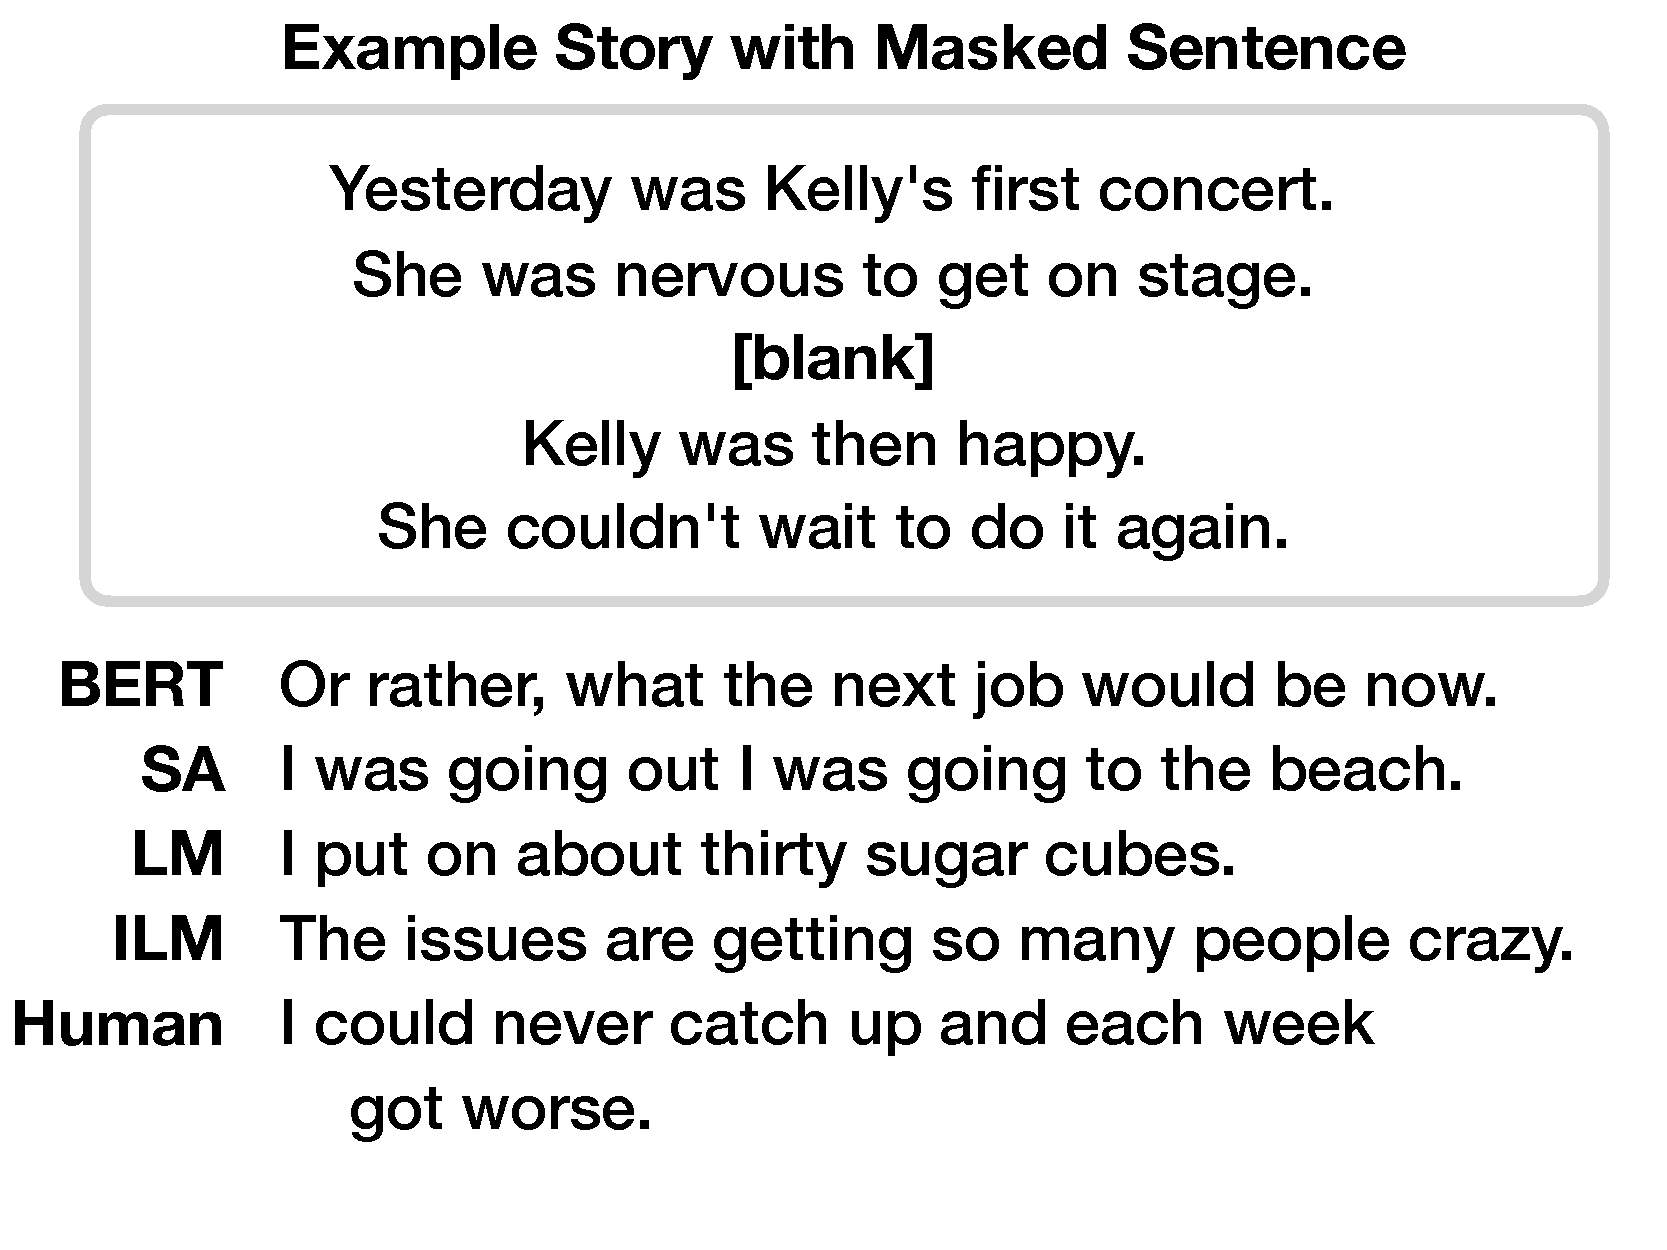
\includegraphics[width=1\linewidth]{figures/ilm_example_story2.pdf}
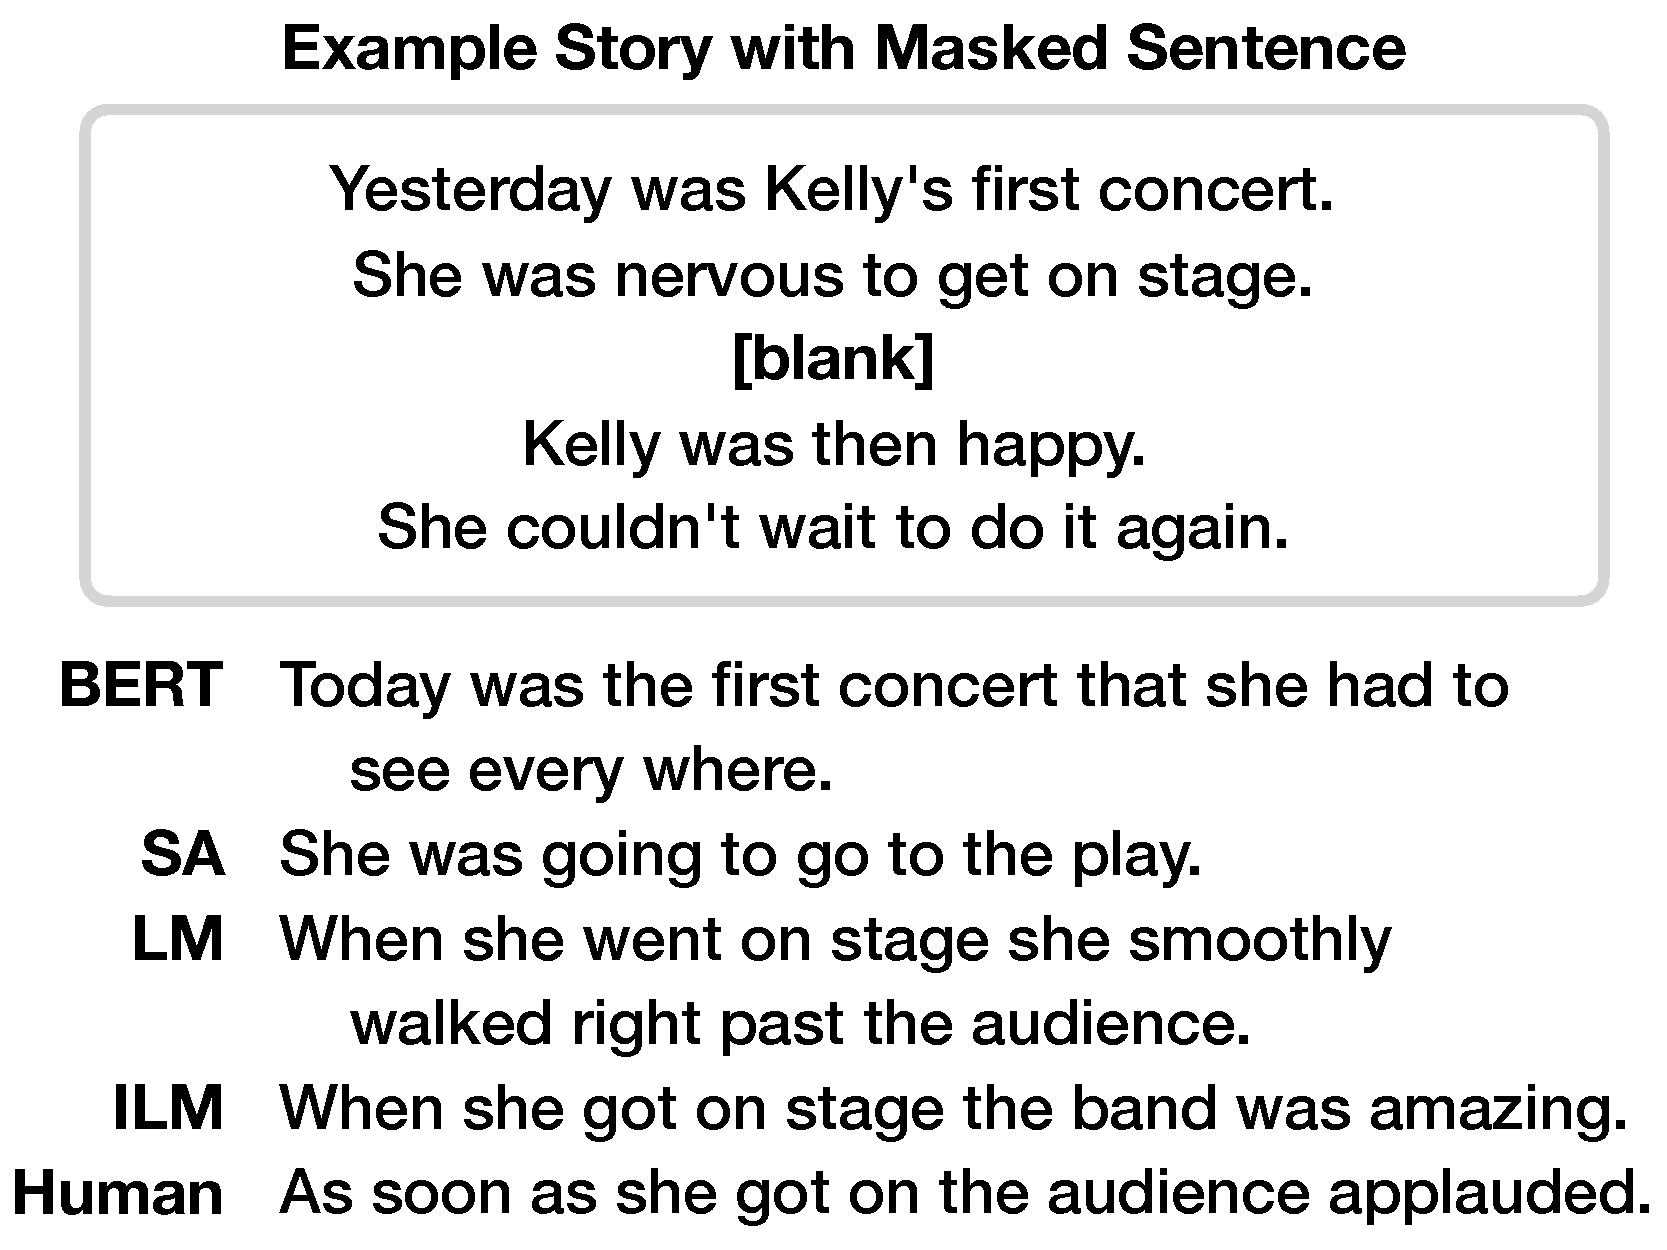
\includegraphics[width=1\linewidth]{figures/ilm_example_story3.pdf}
\caption{Examples of sentence-level infills by different models.}\label{fig:more_examples}
\end{figure}